\documentclass{beamer}
\usepackage[utf8]{inputenc}
\usetheme{Madrid}
\usepackage{amssymb}
\usepackage{pifont}
\usepackage{xcolor}
\usepackage{bigints}
\usepackage{mathrsfs}
\definecolor{dgreen}{rgb}{0.,0.6,0.}
\newcommand{\cmark}{{\color{dgreen}\ding{51}}}%
\newcommand{\xmark}{{\color{red}\ding{55}}}%
\newcommand{\bmark}{{\color{orange}$\sim$}}%


\usepackage{multicol}

\usepackage{amsmath}
\usepackage{cancel}
\DeclareMathOperator*{\argmax}{argmax}
\DeclareMathOperator*{\argmin}{argmin}

\beamertemplatenavigationsymbolsempty
%for backup slides
\newcommand{\backupbegin}{
   \newcounter{finalframe}
   \setcounter{finalframe}{\value{framenumber}}
}
\newcommand{\backupend}{
   \setcounter{framenumber}{\value{finalframe}}
}


\AtBeginSection[
  {\frame<beamer>{\frametitle{Table Of Contents}   
    \tableofcontents[currentsection,currentsection]}}%
]%
{
  \frame<beamer>{ 
    \frametitle{Table Of Contents}   
    \tableofcontents[currentsection,currentsection]}
}


\title[NumKin 2019]{Exponential methods for solving hyperbolic problems with application to kinetic equations}
%\subtitle{Optimisation de WENO pour Vlasov-Poisson}
\author[J. Massot]{N. Crouseilles \inst{1,2} \and L. Einkemmer \inst{3} \and \underline{J. Massot} \inst{2,1}}
\institute[IRMAR]{\inst{1} Inria Rennes -- Bretagne Atlantique \and \inst{2} IRMAR, Université de Rennes \and \inst{3} University of Innsbruck}
\date{\today}

% \defbeamertemplate*{title page}{customized}[1][]
% {
%   \vfill
%   {\usebeamerfont{title}\inserttitle}\par
%   {\usebeamerfont{subtitle}\usebeamercolor[bg]{subtitle}\insertsubtitle}\par
%   \bigskip
%   \vfill
%   \hfill\usebeamerfont{author}\insertauthor\par\par
%   \hfill\textcolor{black}{Encadré par~: Anaïs Crestetto\\\hfill et Nicolas Crouseilles}\par
%   \vfill
%   \hfill\usebeamerfont{date}\insertdate
% }

\begin{document}

\begin{frame}[plain]
  \titlepage
\end{frame}

\begin{frame}{Table Of Contents}
  \tableofcontents
\end{frame}

\section{Vlasov-Poisson equations}
\begin{frame}{Vlasov-Poisson equations 1D$\times$1D}
  Our model: a non-linear transport in $(x,v)\in\Omega\times\mathbb{R}$ of a density distribution $f = f(t,x,v)$:
  $$
    \begin{cases}
      \partial_tf + v\partial_xf + E\partial_vf = 0 \\
      \partial_xE = \int_{\mathbb{R}}f\,\mathrm{d}v
    \end{cases}
  $$
  \begin{itemize}
    \item Filamentation $\rightarrow$ high order methods are needed in phase space $(x,v)$
    \item We want extension to multi-dimensional Vlasov-Poisson. \begin{itemize}\item Easier with FV/FD than splitting strategy\end{itemize}
  \end{itemize}
\end{frame}

\begin{frame}{Fourier transform in $x$ direction}
  $$
    \begin{cases}
      \partial_t\hat{f} + ikv\hat{f} + \widehat{E\partial_vf} = 0 \\
      \hat{E} = -\frac{i}{k}\int\hat{f}\,\mathrm{d}v-1
    \end{cases}
  $$

  Duhamel formula: no CFL in $x$ of the form $\Delta t\leq\sigma\frac{\Delta x}{v_\text{max}}$ with $[-v_\text{max},v_\text{max}]\equiv\mathbb{R}$

  \ 

  \textbf{Toy model} (same difficulties than Vlasov equation):
  $$
    \dot{u} = Au + F(u)
  $$
  $$
    u(t_n+\Delta t) = \exp(\Delta t A)u(t_n) + \underbrace{\int_0^{\Delta t} \exp((\Delta t-s)A)\,F(u(t_n+s))\,\mathrm{d}s}_{\text{needs approximation}}
  $$
  with $\Delta t>0$, $t_n=n\Delta t$ with $n\in\mathbb{N}$.
\end{frame}

\begin{frame}{Idea of \emph{exponential integrators}}
  \textbf{2 strategies:}
  \begin{description}
    \item[exponential Runge-Kutta:] solve exactly what we can and interpolate the other. For example first order exponantial Euler method: $$u(t_n+\Delta t) \approx u^{n+1} = \exp(\Delta tA)u^n + \Delta t\varphi_1(\Delta tA)F(u^n)$$ where $\varphi_1(z) = \frac{(e^z-1)}{z}$

    \item[Lawson:] Change of variable : $v(t):=\exp(-tA)u(t)$ just have to solve $$\dot{v}(t)=\tilde{F}(t,v)=e^{-tA}F(e^{tA}v(t))$$
    For example, Lawson Euler method:
    $$v(t_n+\Delta t) \approx v^{n+1} = v^{n} + \Delta t \exp(-t_n A) F(\exp(t_n A)v^{n})$$
     or as an expression of $u$ : $u^{n+1} = \exp(\Delta t A) u^{n} + \Delta t \exp(\Delta t A) F(u^{n})$.
  \end{description}
\end{frame}

\section{Linear analysis}
\begin{frame}{Reminder on analysis of stability}
  \framesubtitle{\emph{Von Neumann} analysis}
  Approximation of continuous operator:
  $$
    \partial f(x_j) \approx (\mathrm{D}f)_j = \mu f
  $$
  $$f_{j+k} \mapsto e^{ik \varphi}$$ $\mu$: function of $\varphi$: \underline{Fourier symbol}.

  We can only compute Fourier symbol for linear scheme.

  Example for CD2: $$(\partial_xf)_j\approx\frac{f_{j+1}-f_{j-1}}{2\Delta x}\mapsto \frac{e^{i\varphi}-e^{-i\varphi}}{2\Delta x}=\frac{i\sin(\varphi)}{\Delta x}$$
\end{frame}

\begin{frame}{Reminder on analysis of stability}
  \framesubtitle{Stability function}
  For an explicit Runge-Kutta method $RK(s,p)$: \begin{multicols}{2}\begin{itemize}\item $p$: order \item $s$: stages\end{itemize}\end{multicols} we can compute $\dot u = \lambda u$ with: $$u^{n+1} = p(\lambda\Delta t)u^n$$
  where $p$ (\emph{stability function}) is (for eRK) first terms of exponential series of order $p$ plus some terms to the degree $s$: $$p(z) = \sum_{k=0}^p\frac{z^k}{k!}+\sum_{k=p+1}^s\alpha_kz^k$$

  \underline{Stability domain} is define as: $$\mathcal{D}_{(s,p)} = \left\{ z\in\mathbb{C}, |p(z)|\leq 1 \right\}$$
\end{frame}

\begin{frame}{Reminder on analysis of stability}
  \framesubtitle{Geometric interpretation of CFL}
  It is possible to interpret CFL number between time integrator and space method as the biggest homothety ratio that wedges all the amplification factor curve into the stability domain of considered Runge-Kutta methods.

  \begin{columns}
    \begin{column}{0.5\textwidth}
      For example:
      \begin{itemize}
        \item explicit Euler method, stability function:
          $$
            p(z) = z+1
          $$
        \item centered difference scheme of order 2 (CD2), Fourier symbol:
          $$
            \mu = i\sin(\varphi)
          $$
      \end{itemize}
    \end{column}
    \begin{column}{0.5\textwidth}
      \begin{figure}\centering
      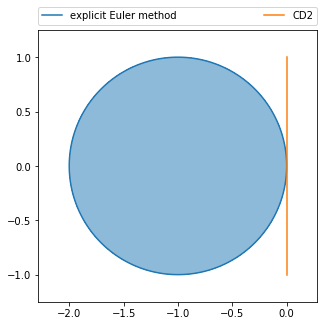
\includegraphics[width=\textwidth]{img/cfl_example.png}
      \end{figure}
    \end{column}
  \end{columns}
\end{frame}

\begin{frame}{Phase discretization}
  \only<1>{
  In $v$ direction we use a DF method :
  \begin{itemize}
    \item CD2 (centred difference of order 2): $(\partial_v\hat{f}_k)(v_j) \approx \dfrac{\hat{f}_{k,j+1}-\hat{f}_{k,j-1}}{2\Delta v}$
    \item WENO5 (weighted essentially non-oscillatory of order 5): $(\partial_xf)_j = \dfrac{f^+_{j+1/2}-f^+_{j-1/2}}{\Delta x}+\dfrac{f^-_{j+1/2}-f^-_{j-1/2}}{\Delta x}$ \begin{itemize} \item WENO5: non linear scheme\dots \xmark \item LW5 (linearized WENO5): linear scheme \cmark\end{itemize}
      $$
        (\partial_v \hat{f}_k)(v_j) \approx \frac{1}{\Delta v}\Big(-\frac{1}{30} \hat{f}_{k,j-3} +\frac{1}{4} \hat{f}_{k,j-2} -\hat{f}_{k,j-1} + \frac{1}{3} \hat{f}_{k,j} +\frac{1}{2} \hat{f}_{k,j+1} - \frac{1}{20} \hat{f}_{k,j+2}\Big)
      $$
  \end{itemize}
  }
  \only<2>{
    \begin{figure}\centering
      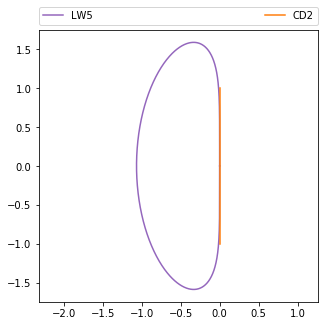
\includegraphics[height=0.8\textheight]{img/weno.png}
    \end{figure}
  }
\end{frame}

\subsection{exponential Runge-Kutta method}
\begin{frame}{ExpRK}
  \only<1>{
    Stability function for ExpRK(2,2):
    $$
      \begin{aligned}
        p(z) = & z^{2} \left(- \frac{e^{\frac{3}{2}i a\Delta t}}{a\Delta t^{2}} + \frac{e^{\frac{1}{2}i a\Delta t}}{a\Delta t^{2}} + \frac{e^{i a\Delta t}}{a\Delta t^{2}} - \frac{1}{a\Delta t^{2}}\right) \\
               & + z \left(- \frac{i e^{\frac{3}{2}i a\Delta t}}{a\Delta t} + \frac{i e^{\frac{1}{2}i a\Delta t}}{a\Delta t}\right) + e^{i a\Delta t}
      \end{aligned}
    $$
    % $$
    %   \begin{aligned}
    %     p(z) = \frac{1}{(a\Delta t)^{2}}\Big[(a\Delta t)^{2} e^{i a\Delta t} &+ i a\Delta t z \left(1 - e^{i a\Delta t}\right) \sqrt{e^{i a\Delta t}} \\
    %                                                                           &- z^{2} \left(\left(e^{i a\Delta t}\right)^{\frac{3}{2}} - \sqrt{e^{i a\Delta t}} - e^{i a\Delta t} + 1\right)\Big]
    %   \end{aligned}
    % $$
    Stability domain depends on $a$ !
  }
  \only<2>{
    \begin{figure}\centering
      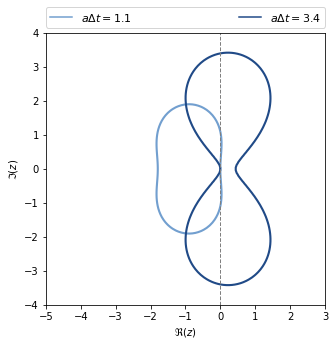
\includegraphics[height=0.7\textheight]{img/expRK22_sd.png}
      \caption{Stability domain of ExpRK(2,2) for $a\Delta t\in\{1.1, 3.4\}$}
    \end{figure}
  }
  \only<3>{
    \begin{figure}\centering
      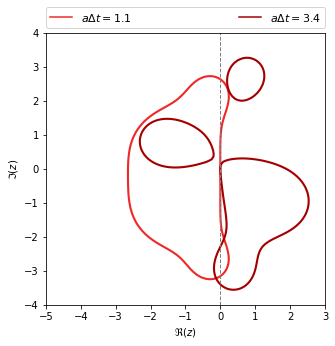
\includegraphics[height=0.7\textheight]{img/CM_sd.png}
      \caption{Stability domain of Cox-Matthews for $a\Delta t\in\{1.1, 3.4\}$}
    \end{figure}
  }
  \only<4>{
    \begin{figure}\centering
      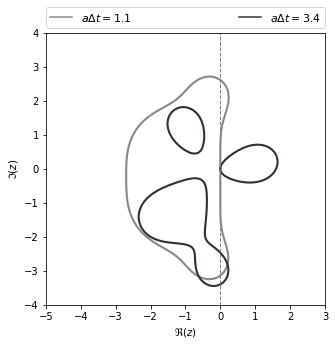
\includegraphics[height=0.7\textheight]{img/K_sd.png}
      \caption{Stability domain of Krogstad for $a\Delta t\in\{1.1, 3.4\}$}
    \end{figure}
  }
  \only<5>{
    \begin{figure}\centering
      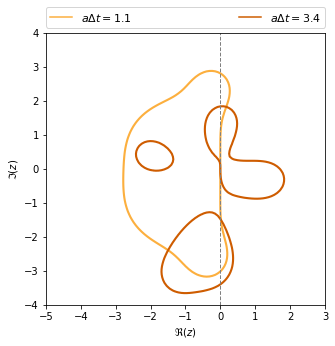
\includegraphics[height=0.7\textheight]{img/HO_sd.png}
      \caption{Stability domain of Hochbruck--Ostermann for $a\Delta t\in\{1.1, 3.4\}$}
    \end{figure}
  }
\end{frame}

\begin{frame}{Stability domain conclusion}
Fourier symbol must fit in the stability domain of ExpRK method \textbf{for each} values of $a\Delta t\in\mathbb{R}$.
  \begin{description}
    \item[\xmark] Impossible with WENO5 (LW5 Fourier symbol) \begin{description}\item[$\rightarrow$] Numerical test: error diverges in very short time\end{description}
    \item[\cmark] Singleton $\{0\}$ is alway in stability domain of ExpRK method for each values of $a\Delta t$
      \begin{description}
        \item[$\rightarrow$] We can try to stabilize it
        \item[\xmark] SPOILER: CFL is equal to zero
      \end{description}
  \end{description}
\end{frame}

\begin{frame}{ExpRK -- CD2}
  Find $y_\text{max}^{exp}(a\Delta t)$ for each value of $a\Delta t$:

  \only<1>{
    \begin{figure}\centering
      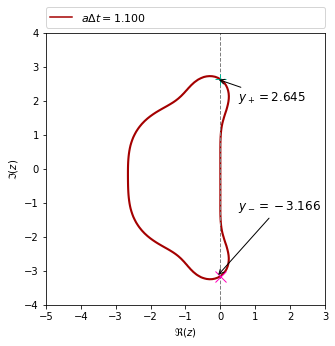
\includegraphics[width=0.5\textwidth]{img/ymax_CM_example1.png}
    \end{figure}
  }
  \only<2>{
    \begin{figure}\centering
      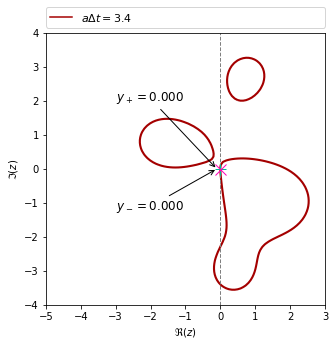
\includegraphics[width=0.5\textwidth]{img/ymax_CM_example2.png}
    \end{figure}
  }

  The CFL of an ExpRK method with CD2 is $y_\text{max}=\min_{a\Delta t}y_\text{max}^{exp}(a\Delta t)$
\end{frame}

\begin{frame}{ExpRK -- CD2}
  \framesubtitle{CFL estimation}

  \only<1>{
    \begin{figure}\centering
      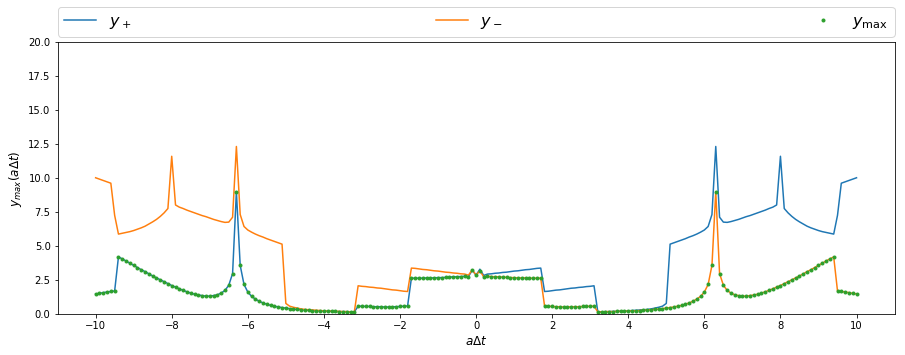
\includegraphics[width=\textwidth]{img/ymax_CM.png}
    \end{figure}
  }
  \only<2>{
    \begin{figure}\centering
      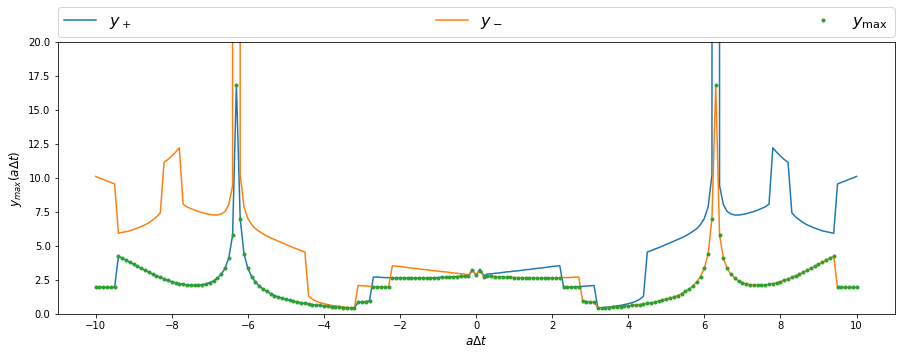
\includegraphics[width=\textwidth]{img/ymax_CM_relax.png}
    \end{figure}
  }
  \only<1>{
    CFL is still equal to 0
  }
  \only<2>{
  Need to relax CFL condition: $\mathcal{D}_\varepsilon = \{z\in\mathbb{C},|p(z)|\leq 1+\varepsilon \}$
  }
\end{frame}

\begin{frame}{ExpRK -- CD2}
  \framesubtitle{CFL relaxation}
  \begin{columns}
    \begin{column}{0.5\textwidth}\centering
      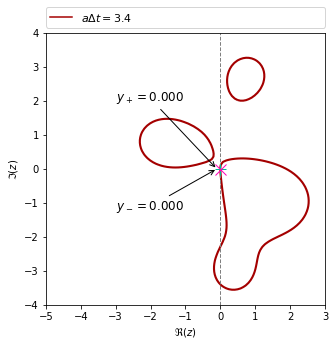
\includegraphics[width=\textwidth]{img/CM_sd_ymax_e0p00.png}
      Cox-Matthews stability domain, relaxation $\varepsilon = 0$
    \end{column}
    \begin{column}{0.5\textwidth}\centering
      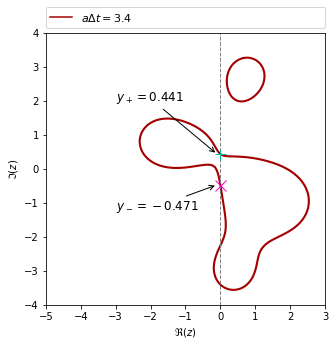
\includegraphics[width=\textwidth]{img/CM_sd_ymax_e0p01.png}
      Cox-Matthews stability domain, relaxation $\varepsilon = 10^{-2}$
    \end{column}
  \end{columns}
\end{frame}

\begin{frame}{ExpRK -- CD2}
  \framesubtitle{CFL estimation}
  \begin{table}
    \centering
    \begin{tabular}{|c|c|c|c|c|}
      \hline
      Methods                                & ExpRK22 & Krogstad & Cox--Matthews & Hochbruck \\
                                             &         &          &               & --Ostermann \\
      \hline
      $y_{\max} (\varepsilon=10^{-3})$ & $0.300$ & $0.100$  & $0.150$      & $0.250$ \\
      \hline
      $y_{\max} (\varepsilon=10^{-2})$ & $0.551$ & $0.200$  & $0.450$      & $0.501$ \\
      \hline  
      $y_{\max} (\varepsilon=10^{-1})$ & $1.001$ & $0.601$  & $1.351$      & $1.702$ \\
      \hline  
    \end{tabular}
    \caption{CFL number, assuming the relaxed stability constraint, for some exponential integrators.}
  \end{table}
\end{frame}

\subsection{Lawson Runge-Kutta method}
\begin{frame}{Lawson}
  For a problem like: $$\dot{u} = Au + F(u)$$
  Stability function of $Lawson(RK(s,n))$ method is:
  $$p_{Lawson(RK(s,n))}(z) = e^{\Delta tA}p_{RK(s,n)}(z)$$

\vfill

  \textbf{\color{blue}BUT:} in our case: $A = ia \in i\mathbb{R}$ so:

  {\hfill Stability domain of $Lawson(RK(s,n))$ is the same than $RK(s,n)$\hfill }

\vfill

  We just loot at $u_t + u_x = 0$ problem.
\end{frame}

\begin{frame}{Lawson -- CD2}
  With CD2, we work only on the imaginary axis, solve:
  $$
    |p(iy)| = 1,\quad y\in\mathbb{R}
  $$
  We can find analytic value while $s<5$ (polynomial roots).

  \begin{table}
    \centering
    \begin{tabular}{|c|c|c|c|}
      \hline
      Methods & Lawson($RK(3,2) \; best$) & Lawson($RK(3,3)$) & Lawson($RK(4,4)$) \\
      \hline
      $y_{\max}$ & $2$ & $\sqrt{3}$ & $2\sqrt{2}$\\
      \hline  
    \end{tabular}
    \caption{CFL number for some Lawson schemes}
  \end{table}
\end{frame}

\begin{frame}{Lawson -- WENO5}
  With WENO we need to numerical estimation

  \only<1>{
    \begin{enumerate}
      \item Evaluate Fourier symbol of LW5 with a fine discrete angular grid $\mu_k = \mu(\theta_k)$ with $\{\theta_k\}\subset [0,2\pi]$. We note $\varphi_k = \arg(\mu_k)$ ($\varphi_k \neq \theta_k$)
      \item A discretized version of the boundary of the stability domain of the underlying Runge-Kutta method is computed.
      \item For each discretized $\mu_k$, we look for the closest boundary point of the Runge-Kutta stability domain. This enables us to compute the associated stretching factor $\sigma(\varphi_k)$.
      \item Taking the minimum over all the discretized eigenvalues yields $\sigma:=\min_k\sigma(\varphi_k)$.
    \end{enumerate}
  }
  \only<2>{
    \begin{figure}\centering
      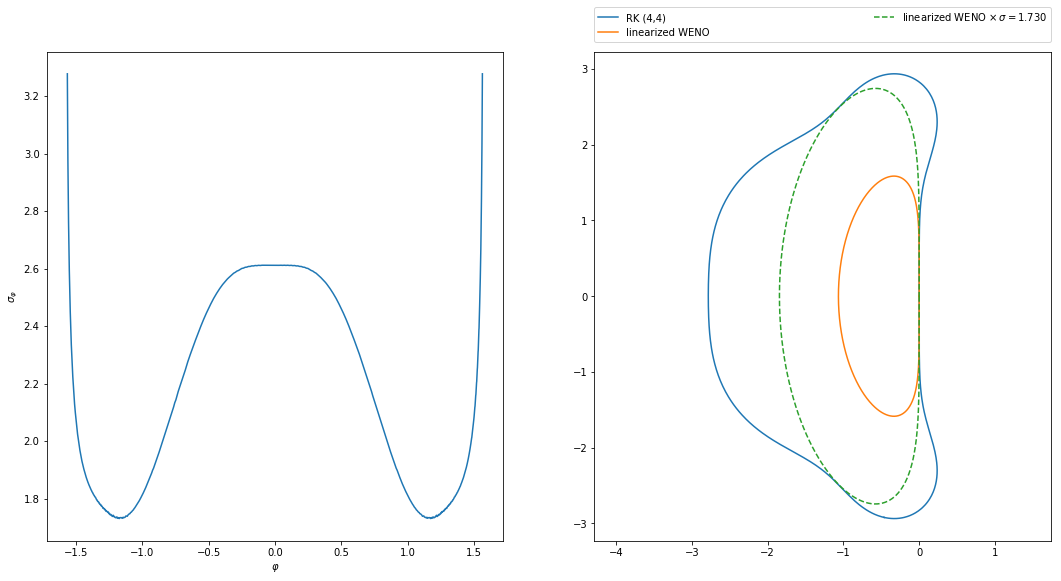
\includegraphics[width=\textwidth]{img/rk44_weno.png}
    \end{figure}
  }
  \only<3>{
    \begin{table}
      \centering
      \begin{tabular}{|c|c|c|c|}
        \hline
        Methods & Lawson($RK(3,2) \; best$) & Lawson($RK(3,3)$) & Lawson($RK(4,4)$) \\
        \hline
        $\sigma $ & $1.344$ & $1.433$   & $1.73$   \\
        \hline  
      \end{tabular}
      \caption{CFL number for some Lawson schemes.}
    \end{table}
  }
\end{frame}

\section{Numerical simulation: Vlasov-Poisson equations}
\begin{frame}{Vlasov-Poisson equation}
  $$
    \begin{cases}
      \partial_tf + v\partial_xf + E\partial_vf = 0 \\
      \partial_xE = \int f\,\mathrm{d}v - 1
    \end{cases}
  $$
  Solve with FFT in $x$ direction, WENO5 or CD2 in $v$ direction, and $Lawson(RK(s,n))$ or ExpRK method in time $t$
\end{frame}
\begin{frame}{Landau damping}
  \only<1>{
    $$
      f(t=0,x,v) = f_0(x,v) = \frac{1}{\sqrt{2\pi}}e^{-\frac{v^2}{2}}(1+0.001\cos(0.5x)),$$
      $x\in[0,4\pi]$, $v\in[-8,8]$, $N_x = 81$, $N_v=128$
  }
  \only<2>{
    \begin{figure}
      \centering
      \resizebox{!}{.7\paperheight}{% GNUPLOT: LaTeX picture with Postscript
\begingroup
  \makeatletter
  \providecommand\color[2][]{%
    \GenericError{(gnuplot) \space\space\space\@spaces}{%
      Package color not loaded in conjunction with
      terminal option `colourtext'%
    }{See the gnuplot documentation for explanation.%
    }{Either use 'blacktext' in gnuplot or load the package
      color.sty in LaTeX.}%
    \renewcommand\color[2][]{}%
  }%
  \providecommand\includegraphics[2][]{%
    \GenericError{(gnuplot) \space\space\space\@spaces}{%
      Package graphicx or graphics not loaded%
    }{See the gnuplot documentation for explanation.%
    }{The gnuplot epslatex terminal needs graphicx.sty or graphics.sty.}%
    \renewcommand\includegraphics[2][]{}%
  }%
  \providecommand\rotatebox[2]{#2}%
  \@ifundefined{ifGPcolor}{%
    \newif\ifGPcolor
    \GPcolorfalse
  }{}%
  \@ifundefined{ifGPblacktext}{%
    \newif\ifGPblacktext
    \GPblacktexttrue
  }{}%
  % define a \g@addto@macro without @ in the name:
  \let\gplgaddtomacro\g@addto@macro
  % define empty templates for all commands taking text:
  \gdef\gplbacktext{}%
  \gdef\gplfronttext{}%
  \makeatother
  \ifGPblacktext
    % no textcolor at all
    \def\colorrgb#1{}%
    \def\colorgray#1{}%
  \else
    % gray or color?
    \ifGPcolor
      \def\colorrgb#1{\color[rgb]{#1}}%
      \def\colorgray#1{\color[gray]{#1}}%
      \expandafter\def\csname LTw\endcsname{\color{white}}%
      \expandafter\def\csname LTb\endcsname{\color{black}}%
      \expandafter\def\csname LTa\endcsname{\color{black}}%
      \expandafter\def\csname LT0\endcsname{\color[rgb]{1,0,0}}%
      \expandafter\def\csname LT1\endcsname{\color[rgb]{0,1,0}}%
      \expandafter\def\csname LT2\endcsname{\color[rgb]{0,0,1}}%
      \expandafter\def\csname LT3\endcsname{\color[rgb]{1,0,1}}%
      \expandafter\def\csname LT4\endcsname{\color[rgb]{0,1,1}}%
      \expandafter\def\csname LT5\endcsname{\color[rgb]{1,1,0}}%
      \expandafter\def\csname LT6\endcsname{\color[rgb]{0,0,0}}%
      \expandafter\def\csname LT7\endcsname{\color[rgb]{1,0.3,0}}%
      \expandafter\def\csname LT8\endcsname{\color[rgb]{0.5,0.5,0.5}}%
    \else
      % gray
      \def\colorrgb#1{\color{black}}%
      \def\colorgray#1{\color[gray]{#1}}%
      \expandafter\def\csname LTw\endcsname{\color{white}}%
      \expandafter\def\csname LTb\endcsname{\color{black}}%
      \expandafter\def\csname LTa\endcsname{\color{black}}%
      \expandafter\def\csname LT0\endcsname{\color{black}}%
      \expandafter\def\csname LT1\endcsname{\color{black}}%
      \expandafter\def\csname LT2\endcsname{\color{black}}%
      \expandafter\def\csname LT3\endcsname{\color{black}}%
      \expandafter\def\csname LT4\endcsname{\color{black}}%
      \expandafter\def\csname LT5\endcsname{\color{black}}%
      \expandafter\def\csname LT6\endcsname{\color{black}}%
      \expandafter\def\csname LT7\endcsname{\color{black}}%
      \expandafter\def\csname LT8\endcsname{\color{black}}%
    \fi
  \fi
    \setlength{\unitlength}{0.0500bp}%
    \ifx\gptboxheight\undefined%
      \newlength{\gptboxheight}%
      \newlength{\gptboxwidth}%
      \newsavebox{\gptboxtext}%
    \fi%
    \setlength{\fboxrule}{0.5pt}%
    \setlength{\fboxsep}{1pt}%
\begin{picture}(7200.00,5040.00)%
    \gplgaddtomacro\gplbacktext{%
      \csname LTb\endcsname%%
      \put(814,704){\makebox(0,0)[r]{\strut{}$-18$}}%
      \put(814,1292){\makebox(0,0)[r]{\strut{}$-16$}}%
      \put(814,1880){\makebox(0,0)[r]{\strut{}$-14$}}%
      \put(814,2468){\makebox(0,0)[r]{\strut{}$-12$}}%
      \put(814,3055){\makebox(0,0)[r]{\strut{}$-10$}}%
      \put(814,3643){\makebox(0,0)[r]{\strut{}$-8$}}%
      \put(814,4231){\makebox(0,0)[r]{\strut{}$-6$}}%
      \put(814,4819){\makebox(0,0)[r]{\strut{}$-4$}}%
      \put(946,484){\makebox(0,0){\strut{}$0$}}%
      \put(1678,484){\makebox(0,0){\strut{}$5$}}%
      \put(2410,484){\makebox(0,0){\strut{}$10$}}%
      \put(3142,484){\makebox(0,0){\strut{}$15$}}%
      \put(3875,484){\makebox(0,0){\strut{}$20$}}%
      \put(4607,484){\makebox(0,0){\strut{}$25$}}%
      \put(5339,484){\makebox(0,0){\strut{}$30$}}%
      \put(6071,484){\makebox(0,0){\strut{}$35$}}%
      \put(6803,484){\makebox(0,0){\strut{}$40$}}%
    }%
    \gplgaddtomacro\gplfronttext{%
      \csname LTb\endcsname%%
      \put(308,2761){\rotatebox{-270}{\makebox(0,0){\strut{}$||E(t)||_{L^2}$}}}%
      \put(3874,154){\makebox(0,0){\strut{}$t$}}%
      \csname LTb\endcsname%%
      \put(5816,4646){\makebox(0,0)[r]{\strut{}Lawson$(RK(4,4))$ - WENO5 $\Delta t = 1/8$}}%
      \csname LTb\endcsname%%
      \put(5816,4426){\makebox(0,0)[r]{\strut{}Lawson$(RK(4,4))$ - WENO5 $\Delta t = 1$}}%
      \csname LTb\endcsname%%
      \put(5816,4206){\makebox(0,0)[r]{\strut{}slope $-0.153$}}%
    }%
    \gplbacktext
    \put(0,0){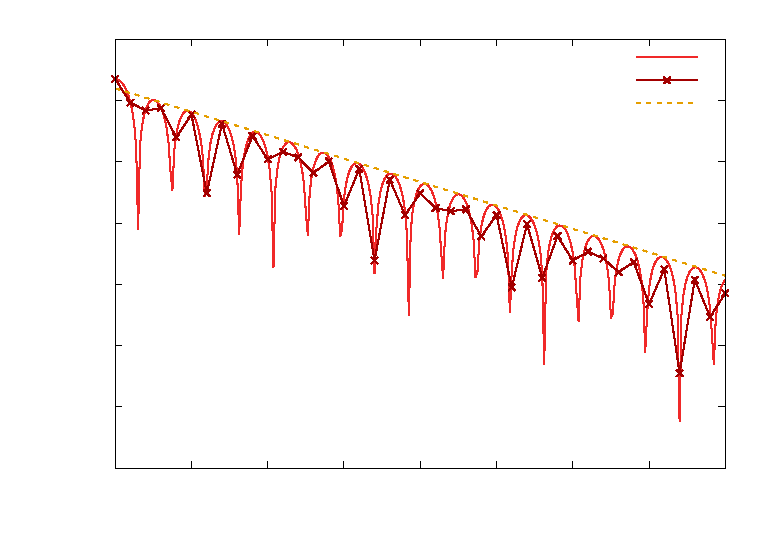
\includegraphics{img/Emax}}%
    \gplfronttext
  \end{picture}%
\endgroup
}
      \caption{Landau damping test: time history of $\|E(t)\|_{L^2}$ (semi-log scale) obtained with Lawson($RK(4, 4)$) and WENO5 
      with $\Delta t=1/8$ and $\Delta t=1$.}
      \label{ld}
    \end{figure}
  }
  \only<3>{
    \begin{figure}
      \centering
      \resizebox{!}{.7\paperheight}{% GNUPLOT: LaTeX picture with Postscript
\begingroup
  \makeatletter
  \providecommand\color[2][]{%
    \GenericError{(gnuplot) \space\space\space\@spaces}{%
      Package color not loaded in conjunction with
      terminal option `colourtext'%
    }{See the gnuplot documentation for explanation.%
    }{Either use 'blacktext' in gnuplot or load the package
      color.sty in LaTeX.}%
    \renewcommand\color[2][]{}%
  }%
  \providecommand\includegraphics[2][]{%
    \GenericError{(gnuplot) \space\space\space\@spaces}{%
      Package graphicx or graphics not loaded%
    }{See the gnuplot documentation for explanation.%
    }{The gnuplot epslatex terminal needs graphicx.sty or graphics.sty.}%
    \renewcommand\includegraphics[2][]{}%
  }%
  \providecommand\rotatebox[2]{#2}%
  \@ifundefined{ifGPcolor}{%
    \newif\ifGPcolor
    \GPcolorfalse
  }{}%
  \@ifundefined{ifGPblacktext}{%
    \newif\ifGPblacktext
    \GPblacktexttrue
  }{}%
  % define a \g@addto@macro without @ in the name:
  \let\gplgaddtomacro\g@addto@macro
  % define empty templates for all commands taking text:
  \gdef\gplbacktext{}%
  \gdef\gplfronttext{}%
  \makeatother
  \ifGPblacktext
    % no textcolor at all
    \def\colorrgb#1{}%
    \def\colorgray#1{}%
  \else
    % gray or color?
    \ifGPcolor
      \def\colorrgb#1{\color[rgb]{#1}}%
      \def\colorgray#1{\color[gray]{#1}}%
      \expandafter\def\csname LTw\endcsname{\color{white}}%
      \expandafter\def\csname LTb\endcsname{\color{black}}%
      \expandafter\def\csname LTa\endcsname{\color{black}}%
      \expandafter\def\csname LT0\endcsname{\color[rgb]{1,0,0}}%
      \expandafter\def\csname LT1\endcsname{\color[rgb]{0,1,0}}%
      \expandafter\def\csname LT2\endcsname{\color[rgb]{0,0,1}}%
      \expandafter\def\csname LT3\endcsname{\color[rgb]{1,0,1}}%
      \expandafter\def\csname LT4\endcsname{\color[rgb]{0,1,1}}%
      \expandafter\def\csname LT5\endcsname{\color[rgb]{1,1,0}}%
      \expandafter\def\csname LT6\endcsname{\color[rgb]{0,0,0}}%
      \expandafter\def\csname LT7\endcsname{\color[rgb]{1,0.3,0}}%
      \expandafter\def\csname LT8\endcsname{\color[rgb]{0.5,0.5,0.5}}%
    \else
      % gray
      \def\colorrgb#1{\color{black}}%
      \def\colorgray#1{\color[gray]{#1}}%
      \expandafter\def\csname LTw\endcsname{\color{white}}%
      \expandafter\def\csname LTb\endcsname{\color{black}}%
      \expandafter\def\csname LTa\endcsname{\color{black}}%
      \expandafter\def\csname LT0\endcsname{\color{black}}%
      \expandafter\def\csname LT1\endcsname{\color{black}}%
      \expandafter\def\csname LT2\endcsname{\color{black}}%
      \expandafter\def\csname LT3\endcsname{\color{black}}%
      \expandafter\def\csname LT4\endcsname{\color{black}}%
      \expandafter\def\csname LT5\endcsname{\color{black}}%
      \expandafter\def\csname LT6\endcsname{\color{black}}%
      \expandafter\def\csname LT7\endcsname{\color{black}}%
      \expandafter\def\csname LT8\endcsname{\color{black}}%
    \fi
  \fi
    \setlength{\unitlength}{0.0500bp}%
    \ifx\gptboxheight\undefined%
      \newlength{\gptboxheight}%
      \newlength{\gptboxwidth}%
      \newsavebox{\gptboxtext}%
    \fi%
    \setlength{\fboxrule}{0.5pt}%
    \setlength{\fboxsep}{1pt}%
\begin{picture}(7200.00,5040.00)%
    \gplgaddtomacro\gplbacktext{%
      \csname LTb\endcsname%%
      \put(990,440){\makebox(0,0)[r]{\strut{}$0.01$}}%
      \put(990,987){\makebox(0,0)[r]{\strut{}$0.1$}}%
      \put(990,1535){\makebox(0,0)[r]{\strut{}$1$}}%
      \put(990,2082){\makebox(0,0)[r]{\strut{}$10$}}%
      \put(990,2629){\makebox(0,0)[r]{\strut{}$100$}}%
      \put(990,3177){\makebox(0,0)[r]{\strut{}$1000$}}%
      \put(990,3724){\makebox(0,0)[r]{\strut{}$10000$}}%
      \put(990,4272){\makebox(0,0)[r]{\strut{}$100000$}}%
      \put(990,4819){\makebox(0,0)[r]{\strut{}$1\times10^{6}$}}%
      \put(1122,220){\makebox(0,0){\strut{}$0$}}%
      \put(1832,220){\makebox(0,0){\strut{}$5$}}%
      \put(2542,220){\makebox(0,0){\strut{}$10$}}%
      \put(3252,220){\makebox(0,0){\strut{}$15$}}%
      \put(3963,220){\makebox(0,0){\strut{}$20$}}%
      \put(4673,220){\makebox(0,0){\strut{}$25$}}%
      \put(5383,220){\makebox(0,0){\strut{}$30$}}%
      \put(6093,220){\makebox(0,0){\strut{}$35$}}%
      \put(6803,220){\makebox(0,0){\strut{}$40$}}%
    }%
    \gplgaddtomacro\gplfronttext{%
      \csname LTb\endcsname%%
      \put(4950,4646){\makebox(0,0)[r]{\strut{}$\frac{\sigma\Delta v}{||E^n||_{L^\infty}}$}}%
      \csname LTb\endcsname%%
      \put(4950,4426){\makebox(0,0)[r]{\strut{}Effective time step}}%
    }%
    \gplbacktext
    \put(0,0){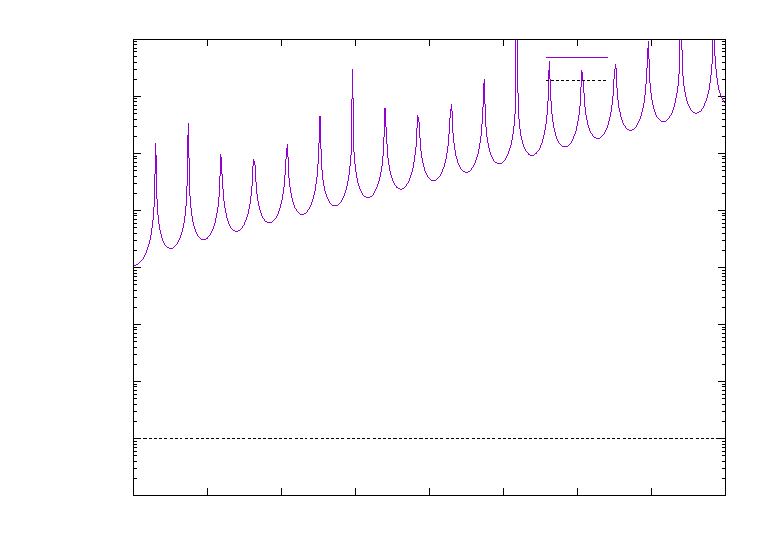
\includegraphics{img/hn}}%
    \gplfronttext
  \end{picture}%
\endgroup
}
      \caption{Landau damping test: time history of the CFL condition (semi-log scale).}
      \label{ld}
    \end{figure}
  }
\end{frame}
\begin{frame}{Bump on Tail (BoT)}
  \only<1>{
    $$f(t=0,x,v) = f_0(x,v) = \left[\frac{0.9}{\sqrt{2\pi}}e^{-\frac{v^2}{2}} + \frac{0.2}{\sqrt{2\pi}}e^{-2(v-4.5)^2} \right](1+0.001\cos(0.5x)),$$
      $x\in[0,20\pi]$, $v\in[-8,8]$, $N_x = 135$, $N_v=256$

    A first simulation with small $\Delta t$ to know: $E_\text{max}\approx 0.6$.

    $$\Delta t = \frac{C\Delta v}{E_\text{max}},\,C=y_\text{max}\text{ or }C=\sigma$$
  }
  \only<2>{
    \begin{figure}
    \centering
        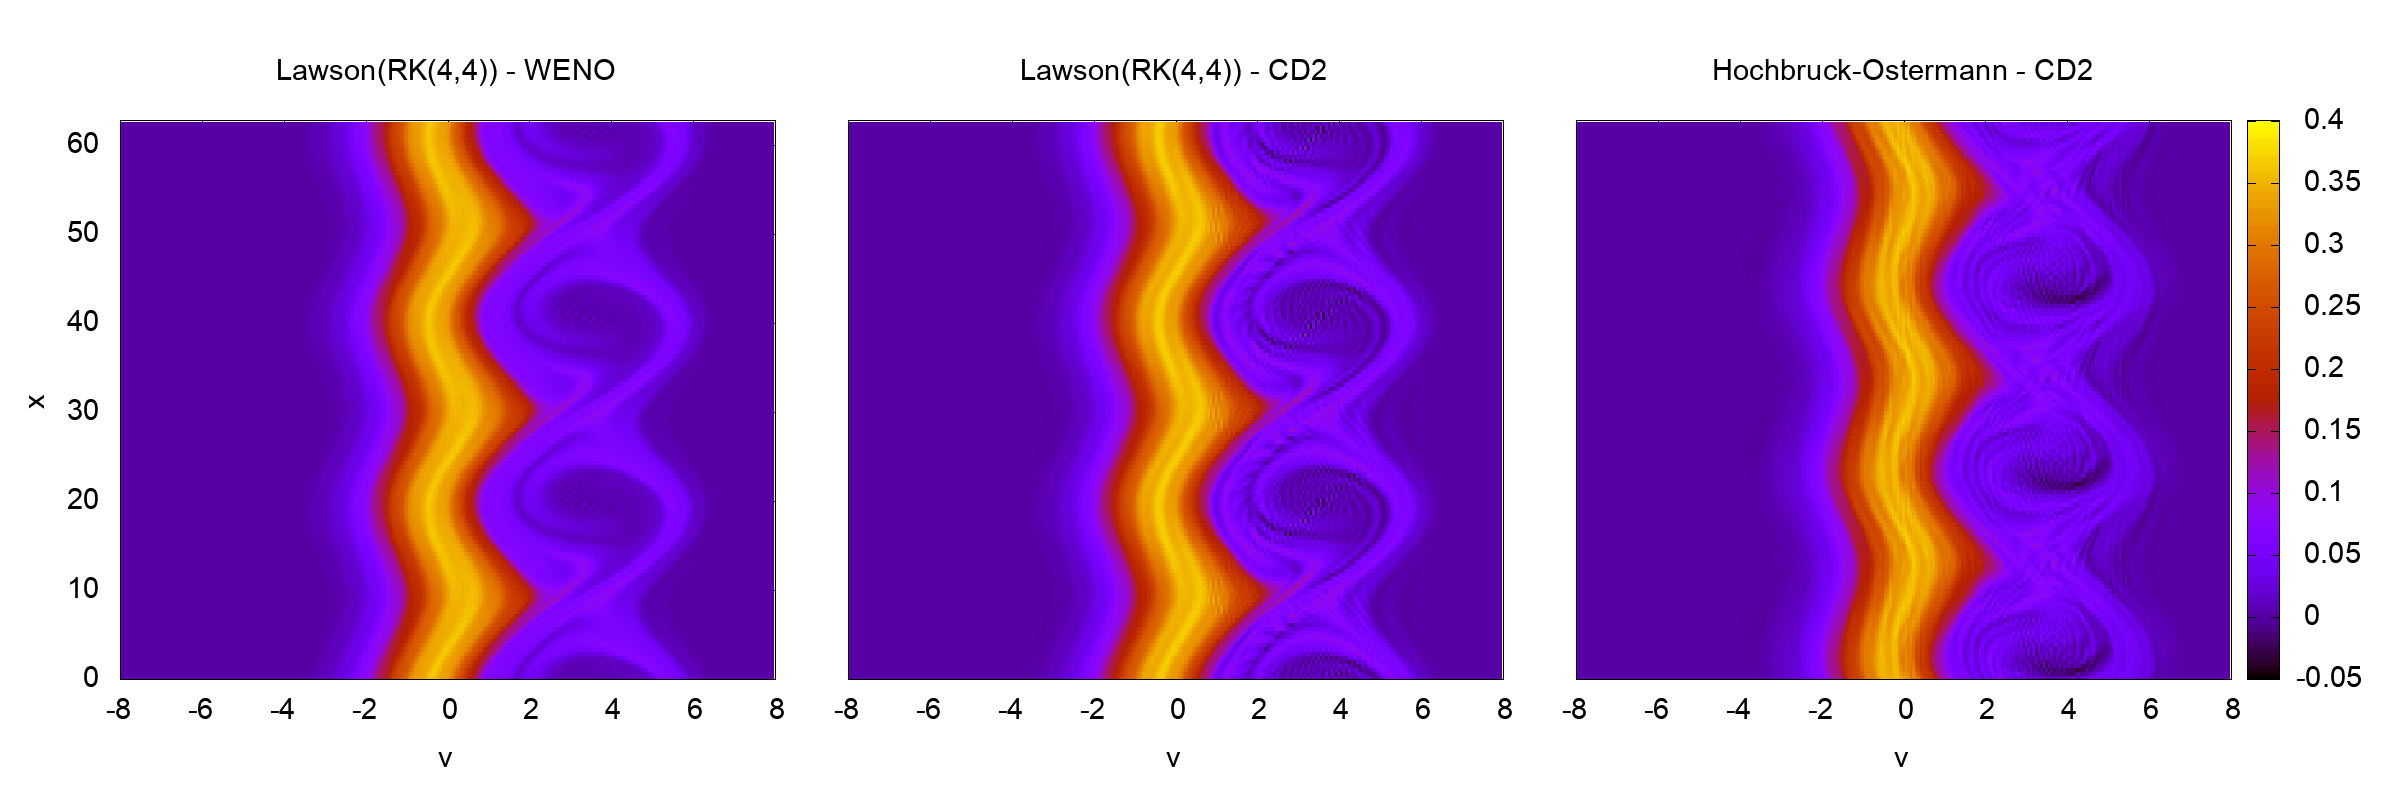
\includegraphics[width=\textwidth]{img/vp_cfl.png}
        \caption{Distribution function at time $t=40$ as a function of $x$ and $v$ for Lawson($RK(4, 4)$) + WENO5 (left), Lawson($RK(4, 4)$) + centered scheme (center), Hochbruck--Ostermann + centered scheme (right).}  
    \label{space}      
    \end{figure}
  }
  \only<3>{
    \begin{figure}
      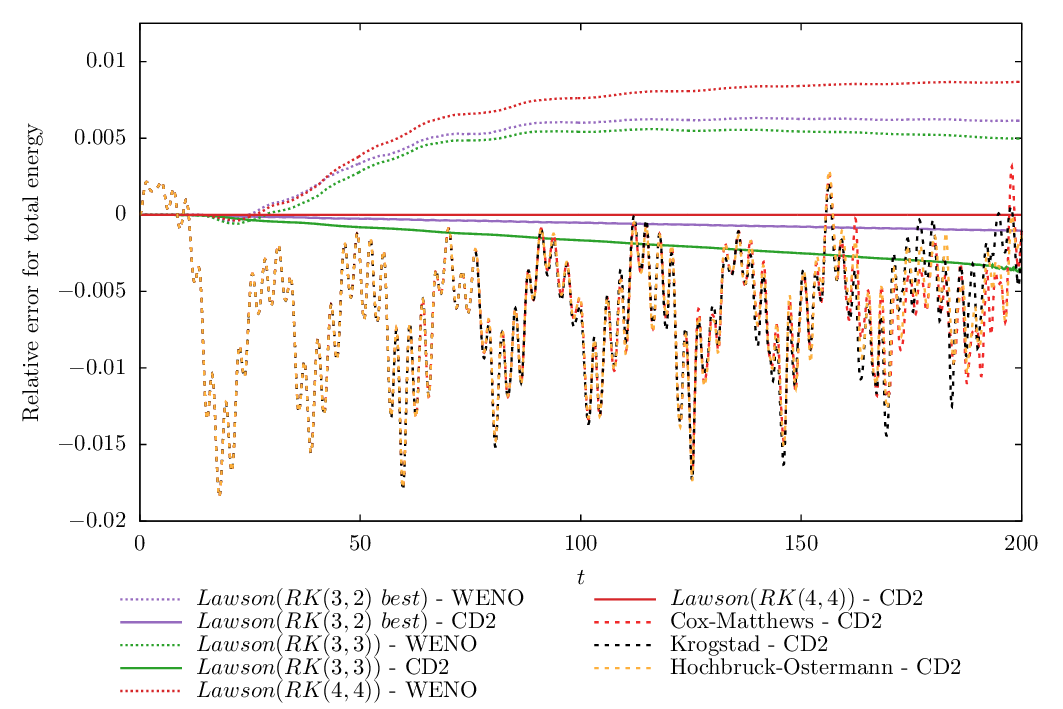
\includegraphics[width=0.9\textwidth]{img/H.png}
      \caption{Time evolution of the relative error of the total energy for the different methods.}
    \end{figure}
  }
  \only<4>{
    \begin{figure}\centering
      \begin{tabular}{cc}
        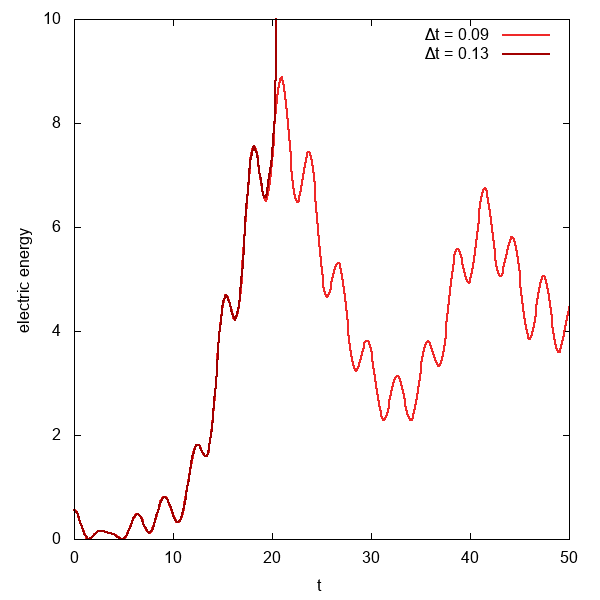
\includegraphics[scale=0.3]{img/ee_weno_rk44.png} &\hspace{-0.2cm}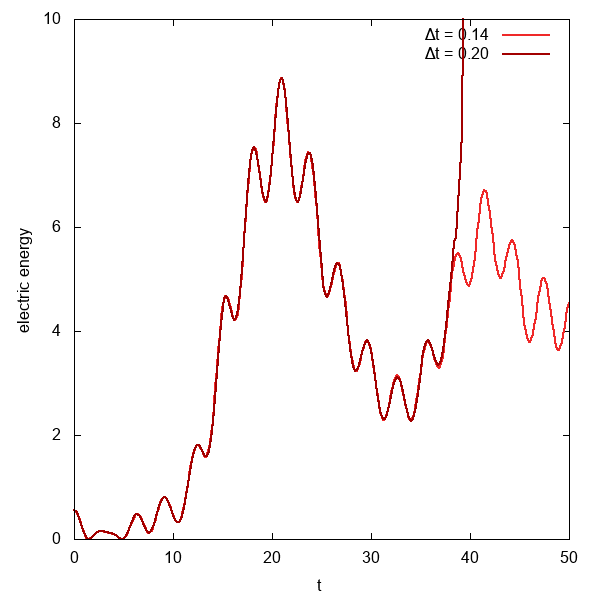
\includegraphics[scale=0.3]{img/ee_o2_rk44.png}
      \end{tabular}
      \caption{Illustration of the accuracy of the CFL estimate obtained from the linear theory. History of electric energy with Lawson($RK(4,4)$) + WENO5 (left),  Lawson($RK(4,4)$) + centered scheme (middle)}
    \end{figure}
  }
  \only<5>{
    \begin{figure}\centering
      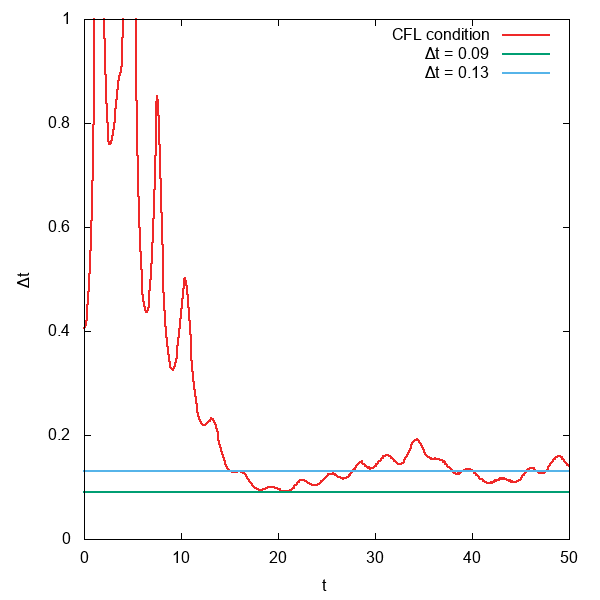
\includegraphics[scale=0.3]{img/bot_cfl_weno_rk44.png}
      \caption{History of CFL condition for Lawson($RK(4,4)$) + WENO5 case (right)}    
    \end{figure}
  }
\end{frame}
\begin{frame}{Adaptive time step size (easy to use)}
  To capture correctly the phenomena involved in the bump on tail test, we take the following time step size:
  $$
    \Delta t_n = \min\left(0.1,\frac{C\Delta v}{||E^n||_{L^\infty}}\right)
  $$
  with $C = y_\text{max}$ or $\sigma$

  $\rightarrow$ Good estimate in practice for Lawson methods.
\end{frame}

\section{Numerical simulation: drift-kinetic equations}
\begin{frame}{Adaptive time step size (error estimate)}
  For adaptive time step size with any time integrator $\varphi$:
  $$
    f^{n+1} = \varphi_{\Delta t_n}(f^n)\qquad;\qquad \tilde{f}^{n+1}=\varphi_{\Delta t_n/2}\circ\varphi_{\Delta t_n/2}(f^n)
  $$
  Richardson extrapolated numerical solution of the method of order $p$:
  $$
    f^{n+1}_R = \frac{2^{p+1}\tilde{f}^{n+1}-f^{n+1}}{2^{p+1}+1}
  $$
  estimate of the local error:
  $$
    e_{n+1} = || f^{n+1}_R - f^{n+1} ||_{L^\infty} + \mathcal{O}(\Delta t_n^{p+2})
  $$
  If $e_{n+1}>\text{tol}$: we reject the step and start again form time $t_n$. Else we determine the new time step size:
  $$
    \Delta t_{new} = s\Delta t_n\left(\frac{\text{tol}}{e_{n+1}}\right)^{1/(p+1)}
  $$
  $s=0.8$ is safety factor.
\end{frame}
\begin{frame}{Drift-kinetic equations}
  $f = f(t,r,\theta,z,v)$
  $$
    \begin{cases}
      \partial_tf - \frac{\partial_\theta\phi}{r}\partial_rf + \frac{\partial_r\phi}{r}\partial_\theta f + v\partial_zf - \partial_z\phi\partial_vf = 0\\
      -\left[ \partial_r^2\phi + \left(\frac{1}{r}+\frac{\partial_rn_0(r)}{n_0(r)}\right)\partial_r\phi + \frac{1}{r^2}\partial_\theta^2\phi \right]+\frac{1}{T_e(r)}(\phi-\langle\phi\rangle) = \frac{1}{n_0(r)}\int_{\mathbb{R}}f\,\mathrm{d}v-1
    \end{cases}
  $$
  $(r,\theta,z,v)\in[0.1,14.5]\times[0,2\pi]\times[0,L]\times\mathbb{R}$,

  Solve with FFT in $z$ direction, CD2 in others
\end{frame}
\begin{frame}{Numerical result}
  \only<1>{
    $$f(t=0,r,\theta,z,v) = f_{\text{eq}}(r,v)\left[1+\epsilon\exp\left(-\frac{(r-r_p)^2}{\delta r}\right)\cos\left(\frac{2\pi n}{L}z+m\theta\right) \right],$$
    where the equilibrium distribution is given by:
    $$
      f_{\text{eq}}(r,v) = \frac{n_0(r)\exp\left(-\frac{v^2}{2T_i(r)}\right)}{(2\pi T_i(r))^{1/2}}
    $$
  }
  \only<2>{
    \begin{columns}
      \begin{column}{0.5\textwidth}
        \includegraphics[width=\textwidth]{img/{snapshots-lawson-rk44-tol1e-2}.pdf}
        Lawson(RK(4,4)) -- CD2
      \end{column}
      \begin{column}{0.5\textwidth}
        \includegraphics[width=\textwidth]{img/{snapshots-coxmatthews-tol1e-2}.pdf}
        Cox-Matthews -- CD2
      \end{column}
    \end{columns}
  }
  \only<3>{
    \begin{figure}\centering
      \includegraphics[height=0.9\textheight]{img/{driftkinetic-tol1.00e-02-64x64x64x128-pert0}.pdf}
    \end{figure}
  }
\end{frame}

\section{Conclusion}
\begin{frame}{Conclusion}
  \begin{itemize}
    \item Better understand on stability of Lawson or ExpRK methods
    \item Automatic script for CFL estimation between Lawson -- CD2 or Lawson -- WENO or ExpRK -- CD2
    \item Adaptive time step size with minimal cost or with an estimate of the local error
  \end{itemize}
\end{frame}
% \begin{frame}{Outlook}
%   \begin{itemize}
%     \item Study hight order Lawson methods (DP5 for example)
%     \item Use explicit embedded Runge-Kutta pair (DP5 for example)
%   \end{itemize}
% \end{frame}

\begin{frame}[t]
  \vfill
  {\usebeamerfont{title} Tank you for your attention}
  \vfill
\end{frame}


\appendix
\backupbegin

\begin{frame}[plain]
  \vspace{0.65\textwidth}
  \hfill\footnotesize{Backup}
\end{frame}

\backupend

\end{document}